% -------------------------------------------------------------------------
%  MusicFormats Library
%  Copyright (C) Jacques Menu 2016-2023

%  This Source Code Form is subject to the terms of the Mozilla Public
%  License, v. 2.0. If a copy of the MPL was not distributed with this
%  file, you can obtain one at http://mozilla.org/MPL/2.0/.

%  https://github.com/jacques-menu/musicformats
% -------------------------------------------------------------------------

% !TEX root = MusicFormatsUserGuide.tex

% -------------------------------------------------------------------------
\chapter{A first example}
% -------------------------------------------------------------------------

Before presenting the \mf\ library in detail, let's get an idea of what it has to offer. The commands used in this chapter will be explained in later chapters.


% -------------------------------------------------------------------------
\section{Raw {\tt xml2ly} usage}
% -------------------------------------------------------------------------

\mxml\ is a textual representation of music scores, that can be produced by scanning score images or exported from GUI scoring applications. It has been designed to facilitate the sharing of scores across applications, which represent scores their own way.

\mf\ provides \xmlToLy\, that converts \mxml\ data to \lily\ code.

In computer science, the simplest example one can write with a language is often named 'Hello World'. \mf\ abides to this rule, suppling \gitmxmlfile{basic/HelloWorld.xml}:
\begin{lstlisting}[language=MusicXML]
jacquesmenu@macmini: ~/musicformats-git-dev/musicxmlfiles > cat basic/HelloWorld.xml
<?xml version="1.0" encoding="UTF-8" standalone="no"?>
<!DOCTYPE score-partwise PUBLIC
    "-//Recordare//DTD MusicXML 3.0 Partwise//EN"
    "http://www.musicxml.org/dtds/partwise.dtd">
<score-partwise version="3.0">
  <work>
    <work-title>Hello World!</work-title>
    </work>
  <!-- A very minimal MusicXML example -->
  <part-std::list>
    <score-part id="P1">
      <part-name>Music</part-name>
    </score-part>
  </part-std::list>
  <part id="P1">
<!--=========================================================-->
    <measure number="1">
  <!-- A very minimal MusicXML example, part P1, measure 1 -->
      <attributes>
        <divisions>1</divisions>
        <key>
          <fifths>0</fifths>
        </key>
        <time>
          <beats>4</beats>
          <beat-type>4</beat-type>
        </time>
        <clef>
          <sign>G</sign>
          <line>2</line>
        </clef>
      </attributes>
  <!-- A very minimal MusicXML example, part P1, measure 1, before first note -->
      <note>
        <pitch>
          <step>C</step>
          <octave>4</octave>
        </pitch>
        <duration>4</duration>
        <type>whole</type>
      </note>
    </measure>
<!--=========================================================-->
  </part>
</score-partwise>
\end{lstlisting}


% -------------------------------------------------------------------------
\section{Redirecting the output and error messages to files}
% -------------------------------------------------------------------------

By default, the \standardOutput\ and \standardError\ are directed to the terminal in which the \xmlToLy\ command has been submitted.

Let's consider the case of \gitmxmlfile{basic/UnknownMaintainerIdentification.xml}:
\begin{lstlisting}[language=Lilypond]
jacquesmenu@macmini: ~/musicformats-git-dev/musicxmlfiles > xml2ly basic/UnknownMaintainerIdentification.xml
*** MusicXML warning *** basic/UnknownMaintainerIdentification.xml:11: creator type "maintainer" is unknown
\version "2.22.0"

% Pick your choice from the next two lines as needed
%myBreak = { \break }
myBreak = {}

% Pick your choice from the next two lines as needed
%myPageBreak = { \pageBreak }
myPageBreak = {}

\header {
    title                = "Hello World!"
    workCreditTypeTitle            = "Hello World!"
    title                = "Hello World!"
}

\paper {
}

\layout {
    \context {
      \Score
      autoBeaming = ##f % to display tuplets brackets
    }
    \context {
      \Voice
    }
}

Part_POne_Staff_One_Voice_One = \absolute {
    \language "nederlands"
    \key c \major
    \numericTimeSignature \time 4/4

    \clef "treble"
    c'1 | % 2
    \barNumberCheck #2
    | % 2
    \barNumberCheck #2
}

\book {
    \score {
        <<

            \new Staff = "Part_POne_Staff_One"
            \with {
            }
            <<
                \context Voice = "Part_POne_Staff_One_Voice_One" <<
                    \Part_POne_Staff_One_Voice_One
                >>
            >>

        >>

        \layout {
            \context {
              \Score
              autoBeaming = ##f % to display tuplets brackets
            }
            \context {
              \Voice
            }
        }

        \midi {
            \tempo 16 = 360
        }
    }

}
Warning message(s) were issued for input line 11
\end{lstlisting}

The \standardOutput\ and \standardError\ streams are merged into the terminal window, which may not be satisfactory.
This behaviour can be changed using the shell's redirection operators:
\begin{itemize}
\item \code{>}: redirects  \standardOutput\ stream to a file;
\item \code{2>}: redirects \standardError\ to a file.
\end{itemize}

Thus, after executing:
\begin{lstlisting}[language=Terminal]
jacquesmenu@macmini: ~/musicformats-git-dev/musicxmlfiles > xml2ly basic/UnknownMaintainerIdentification.xml > output.ly 2> error.txt
\end{lstlisting}

\fileName{output.ly} contains the \lily\ code produced, and \fileName{error.txt} contains:
\begin{lstlisting}[language=Terminal]
jacquesmenu@macmini: ~/musicformats-git-dev/musicxmlfiles > cat error.txt
*** MusicXML warning *** basic/UnknownMaintainerIdentification.xml:11: creator type "maintainer" is unknown
Warning message(s) were issued for input line 11
\end{lstlisting}


% -------------------------------------------------------------------------
\section{The need for options}
% -------------------------------------------------------------------------

Using \xmlToLy\ as in the previous section is somewhat limited. This command:
\begin{lstlisting}[language=Terminal]
jacquesmenu@macmini: ~/musicformats-git-dev/musicxmlfiles > xml2ly basic/MinimalScore.xml > MinimalScore.ly
\end{lstlisting}

leads to this score:\\
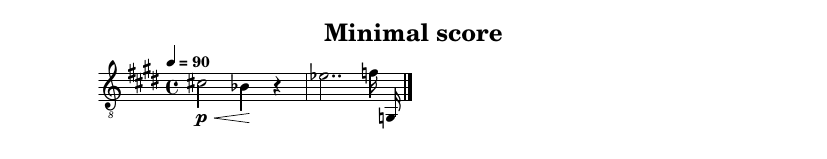
\includegraphics[scale=0.7]{../graphics/MinimalScore.png}

What if we want to change the title in the \lily\ output? This is where options come into play. One of them is \option{query}:
\begin{lstlisting}[language=Terminal]
jacquesmenu@macmini: ~/musicformats-git-dev/musicxmlfiles > xml2ly -query title
--- Help for atom "title" in subgroup "Header"
    -title STRING
          Set 'title' to STRING in the LilyPond code \header.
\end{lstlisting}

Using it this way:
\begin{lstlisting}[language=Terminal]
jacquesmenu@macmini: ~/musicformats-git-dev/musicxmlfiles > xml2ly basic/MinimalScore.xml -title "U. N. Known" > MinimalScore.ly
\end{lstlisting}

produces that score:\\
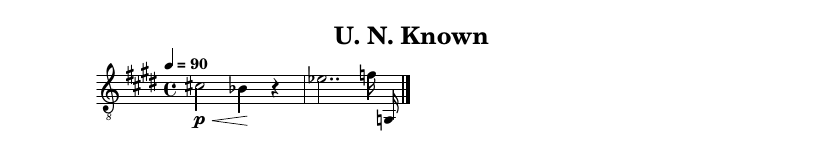
\includegraphics[scale=0.7]{../graphics/MinimalScoreWithAnotherTitle.png}

The effect of the \optionName{title} option is for \xmlToLy\ to generate this at the beginning of the \lily\ output:
\begin{lstlisting}[language=Lilypond]
\version "2.22.0"

% ... ... ...

\header {
    title                = "U. N. Known"
		% ... ... ...
}

% ... ... ...
\end{lstlisting}

We could of course add this \code{title} setting by hand after \xmlToLy\ has produced \lily\ code, but all \mf\ is about is to \MainIt{automate} such things as much as possible.

This is why there are  many options to the \mf\ tools, which in turn explains why \oahRepr, a powerfull options and help handling infrastructure, is provided as part of the library.


% -------------------------------------------------------------------------
\section{The passes at work}
% -------------------------------------------------------------------------

The passes involved in a conversion can be seen with suitable %%%JMI
%the \optionNameBoth{auto-output-file-name}{aofn}, \optionNameBoth{trace-passes}{tpasses} and \optionNameBoth{display-cpu-usage
%}{cpu}
options:
\begin{lstlisting}[language=Terminal]
jacquesmenu@macmini: ~/musicformats-git-dev/musicxmlfiles > xml2ly -auto-output-file-name -trace-passes -display-cpu-usage basic/Anacrusis.xml

%--------------------------------------------------------------
  Handle the options and arguments from argc/argv
%--------------------------------------------------------------
This is xml2ly v0.9.52 (November 29, 2021) from MusicFormats v0.9.60 (January 25, 2022)
Launching the conversion of "basic/Anacrusis.xml" to LilyPond
Time is Thursday 2022-02-03 @ 14:19:32 CET
The command line is:
  xml2ly -auto-output-file-name -trace-passes -cpu basic/Anacrusis.xml
or with options long names:
  xml2ly -auto-output-file-name -trace-passes -display-cpu-usage basic/Anacrusis.xml
or with options short names:
   -aofn -tpasses -cpu basic/Anacrusis.xml
LilyPond code will be written to Anacrusis.ly
The command line options and arguments have been analyzed

%--------------------------------------------------------------
  Pass 1: Create an MXSR from a MusicXML file
%--------------------------------------------------------------
% MusicXML data uses UTF-8 encoding

%--------------------------------------------------------------
  Pass 2a: Create an MSR skeleton from the MXSR
%--------------------------------------------------------------

%--------------------------------------------------------------
  Pass 2b: Populate the MSR skeleton from MusicXML data
%--------------------------------------------------------------

<!--=== part "P1", line 60 ===-->

%--------------------------------------------------------------
  Pass 3: Convert the first MSR into a second MSR
%--------------------------------------------------------------

%--------------------------------------------------------------
  Pass 4: Convert the second MSR into an LPSR
%--------------------------------------------------------------

Opening file 'Anacrusis.ly' for writing

%--------------------------------------------------------------
  Pass 5: Convert the LPSR into LilyPond code
%--------------------------------------------------------------
Timing information:

Activity  Description                                             Kind       CPU (sec)
--------  ------------------------------------------------------  ---------  ---------

          Handle the options and arguments from argc/argv         mandatory    0.02798
Pass 1    Create an MXSR from a MusicXML file                  mandatory    0.00420
Pass 2a   Create an MSR skeleton from the MXSR                    mandatory    0.00191
Pass 2b   Populate the MSR skeleton from MusicXML data            mandatory    0.00314
Pass 3    Convert the first MSR into a second MSR                 mandatory    0.00069
Pass 4    Convert the second MSR into an LPSR                     mandatory    0.00090
Pass 5    Convert the LPSR into LilyPond code                 mandatory    0.00156

Total (sec)  Mandatory  Optional
-----------  ---------  ---------
0.04037      0.04037    0.00000
\end{lstlisting}

The optional passes are those that display \mf\ internal data. They are triggered by suitable options, see \sectionRef{Displaying MusicFormats internal data}.

The resulting \fileName{Anacrusis.ly} file leads to this score where submitted to \lily:\\
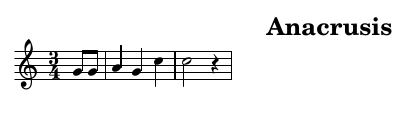
\includegraphics[scale=1]{../graphics/Anacrusis.png}
